\chapter{Projective Geometry}
\label{ch:lesson24}

Chapter~\ref{ch:lesson08} built a hierarchy of 2D transforms --- Euclidean, similarity, affine --- and noted that all three preserve parallel lines. This chapter covers the next, most general step: the \textbf{projective transform (homography)}, which models what a camera actually does when it looks at a flat surface from an angle, and which does \emph{not} preserve parallelism. That's not a bug --- it's exactly the phenomenon of a vanishing point, and it's the tool behind perspective correction and image stitching.

\section{Homogeneous coordinates}

Represent a 2D point $(x,y)$ as a 3-vector $(x,y,1)$. Any $3\times3$ matrix $H$ can then act on it by ordinary matrix multiplication; converting back to 2D means dividing by the third coordinate:
\begin{equation}
\begin{bmatrix}x'\\y'\\w'\end{bmatrix} = H\begin{bmatrix}x\\y\\1\end{bmatrix}, \qquad (x'_{\text{2D}}, y'_{\text{2D}}) = \left(\frac{x'}{w'}, \frac{y'}{w'}\right).
\end{equation}
Two big payoffs: first, a $3\times3$ matrix can represent translation too (impossible with a $2\times2$ matrix alone, which is why Chapter~\ref{ch:lesson08} needed a separate translation vector). Second, that division by $w'$ is what lets a homography model genuine \emph{perspective} effects --- not just the affine transforms of Chapter~\ref{ch:lesson08}, but photos where parallel lines converge toward a vanishing point, exactly what a real camera does when it looks at a flat surface from an angle. Note also that $H$ and $cH$ (any nonzero scalar multiple) represent the \emph{exact same} transform, since the division cancels the scale --- a homography has only 8 independent degrees of freedom, not 9.

\section{Parallel lines stop being parallel}

Extending Chapter~\ref{ch:lesson08}'s hierarchy: an affine matrix has a fixed bottom row $(0,0,1)$; a projective matrix allows any $(g,h,1)$. That's the only difference, and it alone is enough to destroy parallelism, as Figure~\ref{fig:l24-1} shows.

\begin{figure}[h]
\centering
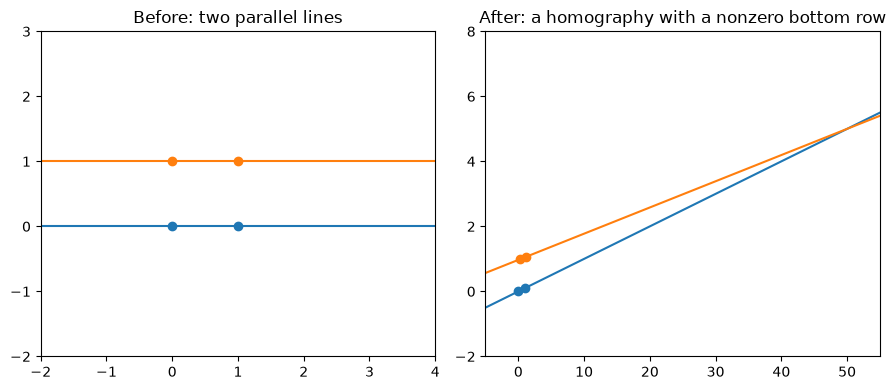
\includegraphics[width=0.85\textwidth]{figures/lesson24_fig01.png}
\caption{Two parallel lines, before and after a homography with a nonzero bottom row --- they now converge toward a vanishing point.}
\label{fig:l24-1}
\end{figure}

\subsection*{Vanishing points, computed two ways}

Where do these two lines actually meet? Intersecting the transformed line segments directly gives $(50, 5)$. More elegantly: transforming the \emph{point at infinity} in the original lines' shared direction $(1,0)$, represented in homogeneous coordinates as $(1,0,0)$, gives the exact same answer, $(50, 5)$ --- confirming that a homography applied to a point at infinity lands exactly on the corresponding vanishing point.

Points aren't the only thing homogeneous coordinates represent elegantly --- a line $ax+by+c=0$ is just as naturally the 3-vector $l=(a,b,c)$, with a point $p=(x,y,1)$ lying on it exactly when $l^\top p=0$. Two useful consequences follow from the cross product: the line through two points is $l=p_1\times p_2$, and the intersection of two lines is $p=l_1\times l_2$ --- both give the same vanishing point, $(50,5)$, computed a third way.

\section{When does a homography actually apply?}

A homography exactly relates two photos in exactly two situations: photographing a flat surface from two different positions, or photographing \emph{any} 3D scene, flat or not, from the same camera position while only rotating the camera between shots. That second case is what makes Chapter~\ref{ch:lesson25}'s panorama stitching work on ordinary, non-planar scenes --- a translating camera or a genuinely 3D scene viewed from two different positions has no single homography that relates the two images exactly.

\section{Perspective correction: rectifying a photographed document}

The most common practical use of a homography: given 4 point correspondences (e.g.\ the 4 corners of a document), \code{cv2.getPerspectiveTransform} solves for the unique homography mapping one set of 4 points to the other, and \code{cv2.warpPerspective} applies it. The trapezoid shape a photographed rectangle takes on --- edges that were parallel in real life visibly converging in the photo --- is called \textbf{keystoning}, and it's exactly the vanishing-point effect above, now applied to a document, as Figure~\ref{fig:l24-2} shows.

\begin{figure}[h]
\centering
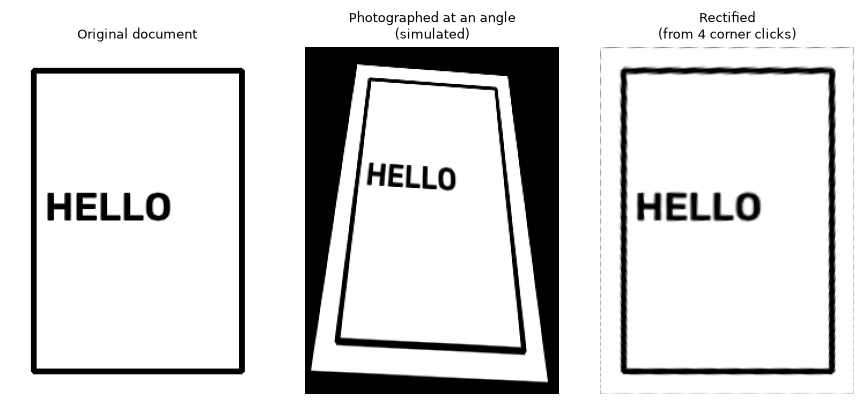
\includegraphics[width=0.85\textwidth]{figures/lesson24_fig02.png}
\caption{A document, a simulated photograph at an angle (strong keystoning), and the rectified result from 4 corner correspondences. Mean absolute pixel difference after the distort-then-rectify round trip is $4.59$ --- small resampling loss only.}
\label{fig:l24-2}
\end{figure}

\section{Solving for a homography from many correspondences}

4 correspondences exactly determine a homography's 8 degrees of freedom, with no slack for error. With \emph{more} than 4 (typically from automatic feature matching, Chapter~\ref{ch:lesson20}), the problem becomes an overdetermined least-squares fit --- the Direct Linear Transform (DLT) algorithm that \code{cv2.findHomography} implements, optionally wrapped in RANSAC (Chapter~\ref{ch:lesson23}) to reject bad correspondences as outliers.

With 30 clean synthetic correspondences: \code{findHomography} recovers the true homography to 4 decimal places, with all 30 points marked as inliers.

\subsection*{RANSAC in practice: homography estimation with bad matches}

With clean correspondences, passing \code{cv2.RANSAC} to \code{findHomography} makes no visible difference --- there's nothing to reject. Injecting 15 deliberately garbage correspondences alongside the 30 genuine ones shows the real effect: RANSAC finds exactly the 30 genuine correspondences (inliers: $30/45$) and reconstructs the homography to a mean reprojection error of $1.49\times10^{-6}$ pixels on the true inliers. A plain least-squares fit on the same contaminated data reaches a mean reprojection error of $1.06\times10^{4}$ pixels --- off by ten orders of magnitude more, effectively useless for anything requiring pixel-level accuracy, because $15$ bad matches out of $45$ ($33\%$) was more than enough to corrupt an unweighted sum-of-squares fit.

\section{Looking ahead: projective geometry in 3D}

Everything in this chapter has been 2D-to-2D: a homography relates two planes (images or flat surfaces in the world). Later chapters extend the same projective machinery one dimension further, deriving the camera's projection matrix that maps a 3D scene onto a 2D image in the first place.

\subsection*{Exercises}
\begin{enumerate}
  \item Add zero-mean Gaussian noise (e.g.\ std 2 pixels) to the second point set before calling \code{cv2.findHomography}. How much does the estimated homography drift from the true one, and does increasing the number of correspondences (say, from 30 to 200) reduce that drift?
  \item Increase the number of injected bad matches from 15 until RANSAC starts to fail. Using the iteration-count formula from Chapter~\ref{ch:lesson23} (minimal sample size 4 for a homography), roughly what outlier fraction is that, and how many iterations would it theoretically require to stay $99\%$ confident of success?
  \item In the vanishing-point demo, change the two lines to be \emph{vertical} instead of horizontal (e.g.\ $x=0$ and $x=1$), and predict, then verify, where their vanishing point ends up using the point-at-infinity trick with direction $(0,1,0)$.
\end{enumerate}

\vfill
\fullcode{lesson24}{lesson24_projective_geometry}
